\documentclass[12pt,preprint]{aastex}
%%\documentclass[manuscript]{aastex}
%%\documentclass[preprint2]{aastex}
%%\documentclass[preprint2,longabstract]{aastex}
\usepackage{graphicx,amsmath,color,natbib,soul,morefloats,longtable,mathrsfs,amsfonts,amssymb,tabularx,rotating,threeparttable,booktabs,caption,fixltx2e,bm}
\bibpunct{(}{)}{;}{a}{}{,}
%%%%%%%%%%%%%%%%%%%%%%%%%%%%%%%%%%%%%%%%%%%%%%%%%%%%%%%%%%%%%%%%%%%%%%%%%%%%%%%%
\newcommand{\myemail}{xuexx@mpia.de}
\newcommand{\DM}{\mathcal{DM}}
\newcommand{\feh}{{\rm [Fe/H]}}
\newcommand{\m}{{\it m}}
\newcommand{\co}{{\it c}}
\newcommand{\ldm}{\mathscr{L}\bigl(\mathcal{DM}\bigr)}
\newcommand{\lph}{\mathscr{L}\bigl({data_i}|p_H\bigr)}
\newcommand{\rgc}{\ensuremath{\mathrm{r}_{GC}}}
\shorttitle{The stellar halo profile of the Milky Way }
\shortauthors{Xue et al.}
%%%%%%%%%%%%%%%%%%%%%%%%%%%%%%%%%%%%%%%%%%%%%%%%%%%%%%%%%%%%%%%%%%%%%%%%%%%%%%%%
\begin{document}
\title{The density profile of the Milky Way's stellar halo to $\rm 80~$kpc}
\author{Xiang-Xiang Xue\altaffilmark{1},Hans-Walter Rix\altaffilmark{1},Zhibo Ma\altaffilmark{2},Heather Morrison\altaffilmark{2},Jo Bovy\altaffilmark{3},Braimir Sesar\altaffilmark{1}}
\altaffiltext{1}{Max-Planck-Institute for Astronomy K\"{o}nigstuhl 17,
D-69117, Heidelberg, Germany}
\altaffiltext{2}{Department of Astronomy, Case Western Reserve
University, Cleveland, OH 44106, USA}
\altaffiltext{3}{Institute for Advanced Study, Einstein Drive, Princeton, NJ 08540, USA}
%%%%%%%%%%%%%%%%%%%%%%%%%%%%%%%%%%%%%%%%%%%%%%%%%%%%%%%%%%%%%%%%%%%%%%%%%%%%%%%%
\begin{abstract}
We present the density profile of SEGUE-2 spectroscopic halo K giants by considering the selection function information. A sample of $\rm \sim2400$ halo K giants up to $\rm 80~$kpc from the Galactic center and its well-understood selection function enable us to get a robust measurement of the shape and radial profile of the Milky Way's stellar halo out to $\rm 80~$kpc. The data show the stellar halo is oblate and its shape has strong dependence on metallicity (i.e. the more metal-poor stars show rounder density profile.). In addition, we find a strong evidence for variations in flattening with radius. After fitting the data to Einasto profile and a broken power-law with a constant halo flattening, we find the best-fitting Einasto profile with an effective radius at $\rm 21~$kpc, a steepness index of $\rm 2.2$, and a flattening (i.e. ratio of minor axis to major axis) of $\rm 0.78$, and the best-fitting broken power-law with an inner slope of $\rm 2.7$ and an outer slope of $\rm 4.2$, together with a break radius at $\rm 30~$kpc and a flattening of $\rm 0.78$. These two best-fitting models are consistent within 1$-\sigma$. Assuming the halo flattening varies with radii, the best-fitting Einasto profile has a smaller effective radius of $\rm 8~$kpc, but a larger steepness index of $\rm 4.6$, and the flattening changing from $\rm 0.5$ at $\rm 10~$kpc to $\rm 0.95$ at $\rm 80~$kpc. Furthermore, the Einasto profile with variable flattening is consistent with the density profiles with a constant flattening within 1$-\sigma$.
\end{abstract}
\keywords{galaxies: individual(Milky Way) -- Galaxy: halo -- Galaxy: stellar content -- stars: K giants}
%%%%%%%%%%%%%%%%%%%%%%%%%%%%%%%%%%%%%%%%%%%%%%%%%%%%%%%%%%%%%%%%%%%%%%%%%%%%%%%%
\section{Introduction}\label{sec:Introduction}
The Milky Way's extended stellar halo contains only a small fraction ($\lesssim 1\%$) of the Galactic stars, but is an important diagnostic of the Milky Way's formation and dark matter distribution. The position-kinematics-abundance substructure in the stellar halo reflects the Galactic formation history, whether halo stars were born \textit{in situ} or are disrupted satellite debris. By now, individual stars are the by far the largest sample of
kinematic tracers with
$10~\mathrm{kpc}\gtrsim \rgc\lesssim 100~\mathrm{kpc}$ (as opposed to globular clusters or satellite galaxies), and are hence the best tracers to determine the mass profile of Milky Way's dark matter halo. It is obvious that kinematic tracer samples should have sizeable membership, cover a wide radial range at good individual distances. But the spatial distribution of the tracers, in particular their radial profile, must be well understood to use such tracers in dynamical inferences. This is perhaps most obvious when considering the \citet{Jeans1915} Equation, even in its simplest version, spherical and isotropic: the tracer
density profile, $\nu (r)$, in particular its logarithmic radial derivative,
$\partial{\ln \nu}/\partial{\ln r}$, scales the inferred enclosed mass, $M(<r)$, almost linearly.
If we do not know the local power-law exponent to better than, say, $25\%$, we cannot
infer the mass to better than $25\%$ irrespective of the size and quality of the kinematic sample. To a somewhat lesser extent, the inferred mass also depends on the flattening of the tracer population. Yet, at present there is little consensus on the shape and the radial profile of the stellar halo.
The most straightforward way to quantify the stellar halo distribution is star counts. However, this method requires large samples of well-understood completeness, so it is often applied to the photometric catalogs. Very early studies adopted star counts to analyze globular clusters\citep{Harris1976}, RR Lyrae variables\citep{Hawkins1984,Wetterer1996}, blue horizontal branch (BHB) stars\citep{Sommer-Larsen1987}, combination of BHBs and RR Lyraes\citep{Sluis1998}, a star sample near the north galactic pole\citep{Soubiran1993}, or K dwarfs\citep{Gould1998}, and found the stellar halo is well fitted by a single power-law ($\nu \approx (distance)^{−-\alpha}$) with index $\alpha$ of $\rm 3\sim3.5$ and flattening of $\rm 0.5\sim1$. However, \citet{Saha1985} found dozens of RR Lyraes are well described by a broken power-law with $\rm \alpha \sim 3$ out to $25~$kpc, and $\rm \alpha \sim 5$ beyond $\rm 25~$kpc.
All of above studies were based on a few hundred objects at most. Recent years, with the development of sky surveys, the sizes of the photometric samples expand more than $\rm 10$ times. \citet{Robin2000} used a wide set of deep star counts in pencil-beam survey at high and intermediate galactic latitudes to model the density profile and found the best-fit density profile with a flattening of $\rm 0.76$, a power index of $\rm 2.44$. \citet{Siegel2002} found $70,000$ stars in seven Kapteyn selected areas are consistent with a power-law density with index of $\rm 2.75$ and flattening of $\rm 0.6$. \citet{Propris2010} made use of BHB stars from the Two-degree Field Quasar Redshift Survey to find that the halo is almost spherical with a power-law index of $\rm \alpha \sim 2.5$ out to $\rm \sim 100~$kpc. \citet{Sesar2011} used $\rm 27,544$ near-turnoff main-sequence stars out to $\rm \sim 35~$kpc selected from Canada-France-Hawaii Telescope Legacy Survey to find the flattening of stellar halo is $\rm 0.7$ and the density distribution is consistent to a broken power low with an inner slope of $\rm 2.62$ and an outer slope of $\rm 3.8$ at the break radius of $\rm 28~$kpc, or an equally good Einasto profile\citep{Einasto1989} with steepness index of $\rm 2.2$ and effective radius of $\rm 22.2~$kpc. \citet{Deason2011} analyzed $\sim 20,000$ A-type photometric stars selected from Sloan Digital Sky Survey data release 8\citep{Ahn2012} and obtained the best-fitting broken power-law density with an inner slope of $\rm 2.3$, and an outer slope of $\rm 4.6$, with a break radius at $\rm 27~$kpc and a constant flattening of $\rm 0.6$. Straight after that, \citet{Deason2014} found a very steep outer halo profile with slope of $\rm 6$ beyond $50~$kpc, and even steeper slopes of $\rm 6\sim10$ at larger radii.
In addition, several pieces of work point to variations of the stellar halo flattening with radius. \citet{Preston1991} found the density distribution for RR Lyraes follow a power-law with $\rm \alpha \sim 3.2$, together with a variable flattening changing linearly from $\rm 0.54$ at center to $\rm 1$ at 20kpc. But, other work \citep{Sluis1998, Sesar2011,Deason2011} found no evidence for flattening, but no evidence for a change with radius.
Position-velocity maps of the stellar halo beyond $\sim 20~$kpc, practically require luminous
post main-sequence (MS) stars, is turn-off or other MS stars are too faint for large-sample spectroscopy. RR Lyraes and BHBs have repeatedly been used as tracers to study the halo density profile, because they have precise distances and are bright enough to be observed at radii out to $\rm \sim 100~$kpc (e.g. X08, Deason, etc..). Yet, such stars, most prevalent in particularly old and metal-poor populations\citep{Bell2008, Xue2011} are known to have a different structure and profile from e.g. RGB stars in the outer halo, that are representative of all halo populations.
K-giants, as tracers common to all relevant halo sub-populations are traces that can both reflect the (mass-weighted) sub-structure, reflecting the formation history, and to probe the halo mass. To this end, it is crucial to construct the halo shape and radial profile in K-giants. \citet{Xue2014} presents a catalog of K giants with unbiased distance estimates, metallicities, velocities and photometric information, drawn from the Sloan Extension for Galactic Understanding and Exploration\citep[][SEGUE]{Yanny2009b}, which contains $\rm \sim 300$ stars beyond $\rm 50~$kpc.
For K giants observed in SEGUE-2, one can understand and model their selection function well. Therefore, it is possible to determine the halo profile and shape in theses tracers, which is the main goal of the paper here.
Specifically, we set out to describe stellar halo distribution, presuming the density is stratified on (oblate) spheroids, with a radial profile from $\rm 10-80~$kpc that can be characterized by simple  functional forms (Einasto profile and broken power-law). We also explore the metallicity dependence of the shape and radial profile of the stellar halo.
In the next section, we lay out the properties and the selection function of the SEGUE K giants. In \S 3, we present the method of fitting a series of parameterized models to SEGUE-2 K giants, explicitly and rigorously considering the selection function. This step is key in obtaining accurate radial profiles. The results for the stellar halo's radial profile and flattening are presented in \S 4, along with an illustration of the metallicity dependence of the shape and radial profile . Finally, \S 5 discusses the comparison between our results and previous work, and implications for dynamical models.
%%%%%%%%%%%%%%%%%%%%%%%%%%%%%%%%%%%%%%%%%%%%%%%%%%%%%%%%%%%%%%%%%%%%%%%%%%%%%%%%
\section{SEGUE-2 K giants and their selection function}\label{sec:Sample_and_SelectionFunction}
The Sloan Digital Sky Survey\citep[SDSS;][]{York2000} is an imaging and spectroscopic survey covering roughly a quarter of the sky, which has both $ugriz$ imaging \citep{Fukugita1996, Gunn1998, Stoughton2002, Pier2003, Eisenstein2011} and low resolution spectra ($\lambda/\Delta \lambda \sim 2000$). SEGUE is one of
the key projects and has two phases named SEGUE-1 and SEGUE-2, which aim to explore the nature of stellar populations from 0.5 kpc to 100 kpc\citep[][and Rockosi et al. in prep.]{Yanny2009b}. The original SEGUE-1 obtained spectra of 240,000 stars with $\rm g=14-20$ to investigate Milky Way structure, and SEGUE-2 spectroscopically observed around 120,000 stars, focusing on the in situ stellar halo of the Galaxy.
To understand the underlying spatial distribution of the K giants on the basis of this sample, we need understand (and account for) the probability that a star of a given luminosity, color and metallicity ends up in the sample, given its direction and distance.
Spectroscopic surveys of the Milky Way are inevitably affected by such selection effects (cf. \citet{Rix2013}),
often referred to as ``selection biases'', which are due to a set of objective and repeatable decisions of what to observe,
necessitated by the survey design. In particular, only a small fraction of the sky was covered by SEGUE plates,
and for most plates only a fraction of stars that satisfy the photometric selection criteria could be targetted with fibers. Finally, not all stars targetted yield spectra good enough to result in a catalog entry, i.e. had S/N high enough to
verify that they are giants and yield a metallicity. \citet{Bovy2012} and \citet{Rix2013} spelled out how to incorporate this selection function in fitting a parameterized model for the stellar density and we follow their approach in this and the next Section.
Both the SEGUE-1and SEGUE-2 surveys targeted halo giant star candidates, using a variety of photometric and proper motions cuts. About 90\% of the final K-giant sample came from objects observed as \textit{l} -color K-giant targets.
The \textit{l}-color is a photometric metallicity indicator for stars in the color range $0.5 < (g-r)_0 < 0.8$, designed to select metal-poor K giants\footnote{https://www.sdss3.org/dr9/algorithms/segue\_target\_selection.php\#S2\_table.}.
Only SEGUE-2 adopted a consistent color-magnitude cut to select K giants throughout its entire survey: $15.5<g_0<18.5$, $r_0>15$, $0.7<(u-g)_0<3$, $0.5<(g-r)_0<0.8$, $0.1<(r-i)_0<0.6$, and $l-color>0.09$, and we restrict our analysis to this category. We also insist that \textit{l}-color K giant candidates have good proper motion measurements with $\le \rm 11~masyr^{-1}$.
But as broadband photometry is a poor main-sequence giant discriminator, not all stars targeted under the above criteria will be giants. The subsequent identification of K-giants is based solely on their spectral properties. As described in \citet{Xue2014}, this requires spectra that have good Mg index and stellar atmospheric parameters determined by the SEGUE Stellar Parameter Pipeline\citep[SSPP;][]{Lee2008a,Lee2008b,Lee2011}, but have no strong G band.
We can now compare the color-magnitude distribution these spectroscopically confirmed K giants
to the analogous distribution of the photometric \textit{l} -color K giant candidates.
Figure~\ref{f:flkgbias} shows these two distribution (as contours and gray-scale, respectively), summed over all SEGUE-2 plates. As in particular the marginalized histograms at the sides of the panels show, these two distributions are nearly indistinguishable: the chance of a photometric candidate being confirmed as a K-giant is independent of color and magnitude. This simplifies the subsequent analysis and is testament to SEGUE-2's consistency of target selection, targeting and spectral analysis.
While the selection function is constant with apparent magnitudes and de-reddened colors, it varies from plate to plate, in particular with the Galactic latitude of the plate. Given the pencil-beam nature of SEGUE survey, it makes sense to specify the selection fraction plate by plate.
For each plate we define the number of spectroscopically confirmed K giant as $N_{spec.}$, and the number of \textit{l} -color K giant candidates in the plate (both those that were targetted, and those that were not) as $N_{phot.}$. Thus, the plate-dependent selection function (shown as Figure~\ref{f:flkgsf}) is given by
\begin{eqnarray}
S(plate) &=& \frac{N_{spec.}}{N_{phot.}}
\end{eqnarray}
As we want to analyze the spatial distribution, we also restrict our sample to SEGUE-2
\textit{l} -color K giants that have sensible distance estimates from \citet{Xue2014}. To eliminate the contamination from disk
component, we cull K giants with $\rm \feh>-1.2$ and $\rm |z|<4~$kpc, which leads to a final sample of $\rm 2413$
l-color K giants. Figure~\ref{f:fkgdistribution} illustrate the basic sample properties: its sky coverage and spatial
distribution without accounting for the selection function, and the metallicity distribution along with the distances
from \citet{Xue2014}. The stars' distribution reflects the pencil-beam pattern of the SEGUE survey; their Galactocentric
distances range from $\rm 7~$kpc to $\rm 85~$kpc; their mean metallicity is $\rm -1.75~$dex, with some being
as metal-poor as $\rm -3.5$.

\section{Modelling the Stellar Halo Density Distribution}\label{sec:Modelling}

We presume that the stellar halo distribution can be sensibly approximated by a spheroidal distribution with a parameterized radial profile and flattening. For this case we spell out a straightforward and rigorous approach to determine the posterior probability distributions for these \textit{halo parameters} in light of the above data, our knowledge of the SEGUE selection function (see Figures~\ref{f:flkgbias}, ~\ref{f:flkgsf} and ~\ref{f:fkgdistribution}), and astrophysical priors on the luminosity function of giants stars. 

\subsection{Functional Forms for the Radial Profile}\label{sec:RadialProfileFunctions}

In this approach, the choice of one, or more, functional forms for the possible stellar density distribution is inevitable. The foremost goal of our analysis is to find the best axisymmetric approximation to the actual spatial distribution, to have a gross description of the halo structure and as input for simple dynamical models. Our basic assumptions, or restrictions, are that we assume 1) the stellar density to be stratified on (oblate) spheroids, 2) the radial profile to be simple or even smooth, and 3) the flattening to be constant or smoothly and monotonically varying. In light of the well-established sub-structure of the stellar these are obviously only approximation. 

The first assumption implies that the stellar profile $\nu_*(x,y,z)$ is only a function of $r_q$,
where 
\begin{equation}
r_q\equiv \sqrt{R^2 + (z/q)^2},
\end{equation}
where $R\equiv \sqrt{x^2+y^2}$ and $q$ is the flattening, in the simplest case constant.

For the functional form of $\nu_*(r_q)$ we resort to two profile families, previously employed.
For one, the Einasto profile \citep{Einasto1989} that is the 3D analog to the S{\'e}rsic's law\citep{Sersic1963} for surface brightnesses, and has been used in this context \citep{Sesar2011,Deason2011,Merritt2006} :
\begin{equation}
\nu_{\star}(r_q) \equiv \nu_0~exp\left\{-d_n\left[\left(r_q/r_{eff}\right )^{1/n}-1\right ]\right\},
\end{equation}
where $ d_n \approx 3n-1/3+0.0079/n, \mbox{ for } n \ge 0.5 \nonumber$,
and $n$ is a concentration index. Flattening and the (here irrelevant) normalization aside, the Einasto profile has two parameters, $r_{eff}$ and $n$.

Alternatively, we consider a broken (or multiply-broken) power law, a form that has been used extensively to described the radial profile of the Galactic stellar halo\citep{Saha1985,Sesar2011,Deason2011,Deason2014}. In most cases the change in the power-law index, 
$d~ln\nu_*/d~ln r$ has been taken as a step function (e.g. \citet{Deason2011}). We adopt:
\begin{equation}
\rm \nu_\star\left(r_q \right )= \left\{\begin{matrix} \rm \nu_0~r_q^{-\alpha_{in}}, & \rm r_q\leq r_{break} \\ \rm \nu_0\times r_{break}^{(\alpha_{out}-\alpha_{in})}\times r_q^{-\alpha_{out}},&\rm r_q>r_{break} \end{matrix}\right.
\end{equation}
In addition to the flattening and normalization, a (singly) broken power-law has three parameters,
$\alpha_{in}, \alpha_{out}, r_{break}$. Of course, this can be generalized to a multiply-broken
power-law, by introducing an additional pair of $\bigl ( \alpha, r_{break} \bigr )$ (cf. \citet{Deason2014}).

\subsection{Halo parameter estimates, explicitly including the Selection Function}\label{sec:ParameterEstimates}

For the parameter estimates, we essentially follow the approach of \citet{Bovy2012} (cf.  \citet{Rix2013}). 
Since we have already good estimates of $\DM$ and $M_r$ for all objects in the sample (\citet{Xue2014}), we treat $(\DM,M_r,\feh,l,b)$ as the observables (rather than $(m_r,c,\feh,l,b)$, as it makes the fitting formalism more intuitive. However, the apparent magnitudes $m_r$ and (dereddened) colors $c$, will appear explicitly in the selection function.  We denote angular selection function as $S(l,b)\equiv S\bigl ( plate (l,b)\bigr )$ (Eq. 1), and the magnitude-color selection function by $S(m(\DM,M_r),c(M_r,\feh))$, expressed in terms of the "observables" above; we denote the priors on absolute magnitude and metallicity as
$p(M_r)$ and $(\feh)$, respectively. Then the expected rate function for finding a star with 
$(\DM,M_r,\feh,l,b)$ in our context is
\begin{eqnarray}
\rm \lambda(M_r,\DM,\feh,l,b|p_H)&=&\rm |J(x,y,z;\DM,l,b)|\times \nu_\star\bigl (r_q(\DM,l,b)|p_H\bigr )\times \\
&&p(M_r)\times p(\feh) \times S(l,b) \times S\bigl ( m(\DM,M_r),c(M_r,\feh)\bigr )\nonumber.
\end{eqnarray}
The Jacobian term $\rm |J(x,y,z;\DM,l,b)|$ accounts for the transformation from cartesian $\rm (x,y,z)$ to the Heliocentric polar coordinates $\rm (\DM, l, b)$. Note that all the SEGUE plates have the same solid angle of $7~deg^2$. When analysing the data plate by plate, the Jacobian term should be $\rm |J(x,y,z;\DM)|$. $\nu_\star\bigl (r_q(\DM,l,b)|p_H\bigr )$ describes the underlying spatial number density of K giants (i.e. halo density profile), in principle from the base to the tip of the giant branch.
 The explicit form for each term in Eq.(2) in the present context is given by:
 
$ |J(x,y,z;\DM)|_{plate} = \Omega_{plate} \cdot \ln10 / 5 \cdot  d^3$,
 where $\Omega_{plate}=7~deg^2$ and $d=10^{\frac{\DM}{5}-2}$~kpc.
\begin{eqnarray}
\rm p(M_r) \propto \left\{ \begin{array}{rl}
\rm 10^{0.32M_r}, &\mbox{\rm if $\rm M_{r~min,obs}<M_r<M_{r~max,obs}$} ~~~~~~~~~~~~~~~~~~~~~~~~~~~~~~~~~~~~~~~~~~~~~~~~~~~~~~~\\
0, &\mbox{ \rm otherwise}~~~~~~~~~~~~~~~~~~~~~~~~~~~~~~~~~~~~~~~~~~~~~~~~~~~~~~~~~~~~~~~~~~~~~~~~~~~~~~~~~~~~
\end{array} \right.\nonumber
\end{eqnarray}
$$
\rm p(\feh) \propto \left\{ \begin{array}{rl}\rm p(\feh)_{obs}, &\mbox{ \rm if $\rm [Fe/H]_{min,obs}<\feh<[Fe/H]_{max,obs}$} ~~~~~~~~~~~~~~~~~~~~~~~~~~~~~~~~~~~\\
0, &\mbox{ \rm otherwise}~~~~~~~~~~~~~~~~~~~~~~~~~~~~~~~~
\end{array} \right.
$$
$$
\rm S(l_{plate},b_{plate})=\left\{ \begin{array}{rl}
\rm \frac{\rm N_{spec.}}{\rm N_{phot.}}, &\mbox{ \rm if in plate} ~~~~~~~~~~~~~~~~~~~~~~~~~~~~~~~~~~~~~~~~~~~~~~~~~~~~~~~~~~~~~~~~~~~~~~~~~~~~~\\
0, &\mbox{\rm otherwise}~~~~~~~~~~~~~~~~~~~~~~~~~~~~~~~~~~~~~~~~~~~~~~~~~~~~~~~~~~~~~~~~~~~~~~~~~~~~~~~~~~~~~~~
\end{array} \right.
$$
$$
\rm S(m(\DM,M_r),c(M_r,\feh))\propto \left\{ \begin{array}{rl}
1, &\mbox{ \rm if $\rm m_{min,obs}<m<m_{max,obs}$ and $\rm c_{min,obs}<c<c_{max,obs}$} ~~~~~~~~~~~~~~~~~~~~~~~~~~ \\
0, &\mbox{ otherwise}~~~~~~~~~~~~~~~~~~~~~~~~~~~~~~~~~~~~~~~~~~~~~~~~~~~~~
\end{array} \right.
$$
The specific functional forms for the stellar halo profiles $\nu_\star\bigl (r_q(\DM,l,b)|p_H\bigr )$
for Einasto, or broken power-law profiles with different flattening profiles are given in the subsequent Sections.

Following \citet{Bovy2012} the likelihood of the data given $p_H$ and the rate function, can be written as
\begin{eqnarray}
\rm \lph &=& \rm c_{\lambda}^{-N_{KG}}\prod \limits_{i=1}^{N_{KG}}\lambda(M_{ri},\DM_i,\feh_i,l_i,b_i|p_H),
\end{eqnarray}
where the normalization $\rm c_\lambda$ is the integral over the volume in $\rm (\DM,l,b,M_r,\feh)$ space.
\begin{eqnarray}
\rm c_\lambda&=&\rm \sum \limits_{i=1}^{N_{plate}} \int\int\int \lambda(M_r,\DM,\feh,l_{plate},b_{plate}|p_H)dM_rd \DM d \feh
\end{eqnarray}
This normalization integral is the most CPU time-consuming part of the parameter estimates; it can be computed efficiently using Gaussian quadrature rule. We adopt $48\times20\times20$ transformation points in $\DM, ~M_r ~and ~\feh$ space, and then the parameter-independent parts such as Jacobian term, priors of luminosity and metallicity and selection function can be pre-computed on a dense grid. We then vary the $p_H$ to sample the parameter PDF, using emcee\citep{Foreman2013}.

\section{Results}\label{sec:Results}
In this section, we present the results of applying the approach from \S 3 to the sample of \S 2.  
We first focus on the radial profiles, fitting for a radially constant flattening, and taking halo giants of all metallicities. We then show how these results compare for subsamples of different metallicities, and explore radial variations of the flattening, and their impact on the radial profile estimate. The results are summarized in Table 1. 

\subsection{Radial profile at constant flattening}\label{sec:Results_RadialProfile}

Figure~\ref{f:feinasto} presents the fit results for the Einasto profile,  showing the \textit{PDF}s of the three parameters: $r_{eff}=21\pm1~kpc$, $\rm q=0.78\pm0.02$, and $n=2.2\pm0.3$.
To get a sense whether this best fit provides a sensible representation of our data, we compare
 in Figure~\ref{f:fpdm} the distribution of the $\DM$s in the sample to that predicted by the best-fit model. The distributions are summed over all survey directions in both cases, and the overall match is very good. 

Figure~\ref{f:fbpl} shows the analogous results for a broken power-law: we find an inner slope of $\rm \alpha_{in}=2.7\pm0.1$, an outer slope of $\rm \alpha_{out}=4.2\pm0.2$, and a break radius of
 $\rm r_{break}=30\pm3~$kpc, together with a flattening of $\rm q=0.78\pm0.02$. The flattening is consistent with that of the best-fit Einasto profile. The broken power-law profile also predicts a consistent $\rm p(\DM)$ to the observation (shown as Figure~\ref{f:fpdm}).
 
As \citet{Deason2014} claimed much more rapid drop of the stellar density (in BHB stars) beyond $\rm 50~$kpc, we also fit triple power-laws with parameters  ($\alpha_{1},~\alpha_{2}$,~$\alpha_{3}$,~q), that denote the three slopes and flattening, along with the fixed break radii at $r_{break1}=\rm 30~kpc$ and $r_{break2}=\rm 50~kpc$. We find the best inner slope $\rm \alpha_{1}$ is $\rm 2.7$, the middle slope is equal to the outer slope ($\rm \alpha_{2}~=~ \alpha_{3}~=~4.2$), and the flattening $\rm q$ is still $\rm 0.78$, i.e. no evidence of strong drop beyond $\rm 50~$kpc.

How these fits using different functional forms compare, in particular in their logarithmic slopes as a function of radius, we discuss in Section \ref{sec:ModelComparison}.

\subsection{Metallicity-dependence of radial profile and flattening}\label{sec:Results_Flattening}

As some parts of the halo have presumably formed 'in situ', while other parts were accreted from satellites, i.e. through different formation paths that may be reflected in their metallicities, 
 we may expect that the overall spatial structure of the halo depends on metallicity.
To explore any metallicity-dependence of the flattening and radial profile, we split our sample
by metallicity \ into three almost equally size sub-samples. We then fit Einasto profiles with fixed $n=2.2$ to these sub-samples to obtain the best-fit parameters $\rm q ~and ~r_{eff}$. The results of these fits are shown in Figure~\ref{f:ffehdependence}. The three sub-samples have very similar effective radii ($\rm r_{eff}\sim20~$kpc), but the less metal-poor stars ($\rm q\sim0.7$) appear
significantly flatter than the more metal-poor stars ($\rm q\sim0.85$).
So, while the shape of the halo varies somewhat with metallicity, there is no significant overall metallicity gradient in the halo ($\ge 10$~kpc). 

\subsection{Radial variation of halo flattening}\label{sec:Results_FlatteningVariations}
\citet{Preston1991} found the evidence for the increase of flattening with radii. Besides, several pieces of work also tested the variation of halo flattening, but did not find the evidence for it\citep{Sluis1998,Sesar2011,Deason2011}. Both \citet{Preston1991} and \citet{Sluis1998} assumed the profile of halo flattening by themselves. Until now, there is no work to study the exact formula of the variation of halo flattening. The above fits were restricted to radially constant flattening $q$. As there is considerable evidence that at least the innermost part of the halo is quite flattened \citep{Carollo2010}, we explore how our sample can inform us about radial variations in the flattening of the stellar halo.  Instead of assuming $q=~const.~$, we fit the following three expressions for $\rm q(r)$:
\begin{equation}
\rm q\left(r\right)=q_{inf}-\left(q_{inf}-q_0\right)exp\left(1-\frac{\sqrt{r^2+r_0^2}}{r_0}\right),
\end{equation}
where  $\rm q_0$ is the flattening at center, changing to $\rm q_{inf}$ at large radii, with $\rm r_0$ is the (here, exponential) scale radius, over which the change of flattening occurs. This exponential flattening is our assumption. 

Alternatively, we use a functional form that has been used by \citep{Osipkov1979} and \citep{Merritt1985} in a somewhat different context
\begin{equation}
\rm q\left(r\right)=\sqrt{q_0^2+\left(q_{inf}^2+q_0^2\right)\frac{r^2}{r^2+r_0^2}},
\end{equation}
and finally 
\begin{equation}
\rm q\left(r\right)=q_0\sqrt{\frac{r^2+r_0^2}{q_0^2r^2+r_0^2}}
\end{equation}
following \citet{Sluis1998}, which we dub Sluis-Arnold flattening. 
Note that the flattening in all these cases is a function of the spherical radius, $r$, not of $r_q$.

We restrict the possible radial profile Einasto models with above three forms of varying flattening to the data. For all three flattening profiles, we find that the halo is far more flattened at small radii $\bigl ( q(r=10\rm~kpc)\approx 0.6\bigr )$, becomes nearly round beyond  $\rm r_0\approx 30$~kpc)  to $\rm q_{inf}\approx 0.95$),  and that formally small Einasto scale radii are favored ($\rm r_{eff} \sim 10~$kpc). Flattening profiles that correspond to samples of the parameter's PDFs are illustrated Figure~\ref{f:fqv}: the flattening profile depends little on the functional form chose in the modelling. The results are summarized in Table 1.   

Note that while the formal $\rm q_0\approx 0.3$ (at $r=0$~kpc), we have not used any data within $r=10$~kpc. 

The change in $\rm r_{eff}$, when allowing for variable flattening, may seem dramatic. Yet,
the implied radial profile is actually not very different, as we will show below (Section \ref{sec:ModelComparison}).

\subsection{Comparison of Different Functional Forms for the Radial Profile}\label{sec:ModelComparison}

Analogous to the comparison of the flattening profiles shown in Figure~\ref{f:fqv} 
(cf Section \ref{sec:Results_FlatteningVariations}) we now explore how different the 
actual radial density profiles implied by the various fits above actually are over the radial range where they are constrained by data ($10~\rm kpc \le \rm r \le 80~\rm kpc$). Here, we focus
on the local slope of the density profile, i.e. the local power-law exponent, $\rm \frac{dln\nu}{dlnr}$, because of its important role in mass estimates $\rm M(<r)$, e.g. through the Jeans Equation (cf. Section \ref{sec:Introduction}). Since the stellar halo density distributions we consider here are axisymmetric, effectively oblate, we take an intermediate axis (in cylindrical coordinates) as the radial coordinate 
in such comparison, $\rm \frac{dln\nu(R,R/\sqrt{2})}{dlnR}$.

We start by comparing the Einasto profiles with different forms of flattening variation: the upper panel of Figure~\ref{f:fdensity} shows that all three functional forms for the flattening also have  consistent density profiles. Since the Einasto profiles with different definitions of flattening variation are consistent, we will only use the model with exponential flattening to compare with the models with constant flattening. Figure~\ref{f:fdensity} (lower panel) compares  the radial profiles between the models with constant or variable flattening: remarkably the Einasto profiles with constant (black) and variable (blue) flattening have consistent radial profile slopes,
$\rm \frac{dln\nu(R,R/\sqrt{2})}{dlnR}$, despite their quite different $r_{eff}$.
However, the broken power-law profile slope differs significantly from the Einasto profile beyond 50~kpc.

\section{Summary and Discussion}\label{sec:Discussion}
In this paper, we have presented an analysis of the overall spatial distribution of stars in the Galactic halo in the range $10~\rm kpc < r < 80~kpc$, based on over 2,000 spectroscopically confirmed (\textit{l}-color) K-giants from SEGUE-2 with $\rm -3.5<\feh<-1.2$. 
This sample is comparable in size and distance range to previous samples of BHB stars in the Galactic halo, but has the advantage that K-giants
are ubiquitous and well-understood tracers of all stellar halo populations across the relevant age and metallicity range.  We have laid out a formalism for fitting parameterized models to the spatial distribution of these halo stars that quite rigorously accounts for the selection function of the spectroscopic survey. 

We consider a variety of parameterized functional forms for the stellar density distributions
with spheroidal density stratifications. These have either  Einasto or broken power-law profiles 
in radius, and have constant or radially variable flattening. 

We find that the radial distribution can be reasonably well described by either an Einasto profile or a (once) broken power-law. If the flattening is assumed to be constant, the halo is overall mildly oblate. We find that a single power-law is clearly ruled out, as the locally determined power-law slope (for either Einasto, or a broken power law) from $-2.5$ at 15~kpc to $-4.5$ at 50~kpc. In the radial profile of the K-giants, we found no evidence for a second power-law break at 50~kpc, as seen for the BHB stars \citep{Deason2014}. Overall, the halo profile slope
$\rm \frac{dln\nu(R,R/\sqrt{2})}{dlnR}$ seen in the K-giants is significantly shallower than than the one measured and claimed for BHB stars \citep{Deason2014}; whether that is a true discrepancy, or just implies that the population in which BHB stars are more common has 
a steeper profile is not clear.  At any rate, the new, improved information on the radial profile of the stellar halo presented here, should enable better halo mass estimates with stellar kinematics, as the radial profile uncertainties are a more important error source than the velocity dispersion measurements. 

The large sample size and good metallicity estimates ($\delta\feh \approx 0.2$) allow us to 
search for an abundance dependence of the overall halo profile: we find little dependence of the radial profile (e.g. $10\%$ in $r_{eff}$) on metallicity in the range
$\rm -3.5<\feh<-1.2$. 

We also explore the shape (i.e. the flattening) of the radial profile. Presuming radially constant flattening ($q=0.78\pm 0.02$ for the entire sample), we find that the most metal-poor sub-population of the halo $\feh<-1.9$ is considerably less flattened ($q=0.85$) than the rest ($q=0.7$).
We find a distinct radial dependence of the flattening in the observed radial 
range, rising from $q\approx 0.6$ at 10~kpc to $q\approx 0.95$ at 30~kpc and beyond. 
This may reflect the transition from  the \textit{in situ} formed portion halo to accreted halo stars.
Our finding is consistent with early claims \citet{Preston1991} that the halo becomes rounder 
at large radii, but is inconsistent with findings of \citet{Sluis1998, Sesar2011,Deason2011}.
This radial variation may reconcile our (constant) flattening $q=0.78$,
which is less flat than the values found by \citet[;q=0.7]{Sesar2011} 
and \citet[;q=0.58]{Deason2011} : if $q$ varies radially, then the details of the radial weighting matter in the fitting of $q=~\rm const.$ models.



\acknowledgments
The research has received funding from the European Research Council under the European Union's Seventh Framework Programme (FP 7) ERC Grant Agreement n. [321035].
X.-X. Xue acknowledges the Alexander von Humboldt foundation for a fellowship
Funding for SDSS-III has been provided by the Alfred P. Sloan
Foundation, the Participating Institutions, the National Science
Foundation, and the U.S. Department of Energy Office of Science. The
SDSS-III web site is http://www.sdss3.org/.
SDSS-III is managed by the Astrophysical Research Consortium for the
Participating Institutions of the SDSS-III Collaboration including the
University of Arizona, the Brazilian Participation Group, Brookhaven
National Laboratory, University of Cambridge, Carnegie Mellon
University, University of Florida, the French Participation Group, the
German Participation Group, Harvard University, the Instituto de
Astrofisica de Canarias, the Michigan State/Notre Dame/JINA
Participation Group, Johns Hopkins University, Lawrence Berkeley
National Laboratory, Max Planck Institute for Astrophysics, Max Planck
Institute for Extraterrestrial Physics, New Mexico State University,
New York University, Ohio State University, Pennsylvania State
University, University of Portsmouth, Princeton University, the
Spanish Participation Group, University of Tokyo, University of Utah,
Vanderbilt University, University of Virginia, University of
Washington, and Yale University.
This work was made possible by the support of the Max-Planck-Institute
for Astronomy, and supported by the National Natural Science
Foundation of China under grant Nos. 11103031, 11233004, 11390371 and 11003017,
and supported by the Young Researcher Grant of National Astronomical
Observatories, Chinese Academy of Sciences. This paper was partially
supported by the DFG's SFB-881 grant `The Milky Way System'.
%%%%%%%%%%%%%%%%%%%%%%%%%%%%%%%%%%%%%%%%%%%%%%%%%%%%%%%%%%%%%%%%%%%%%%%%%%%%%%%
\bibliographystyle{apj}
\bibliography{refkg}
\clearpage
%%%%%%%%%%%%%%%%%%%%%%%%%%%%%%%%%%%%%%%%%%%%%%%%%%%%%%%%%%%%%%%%%%%%%%%%%%%%%%%%

%%Figure
\begin{figure}
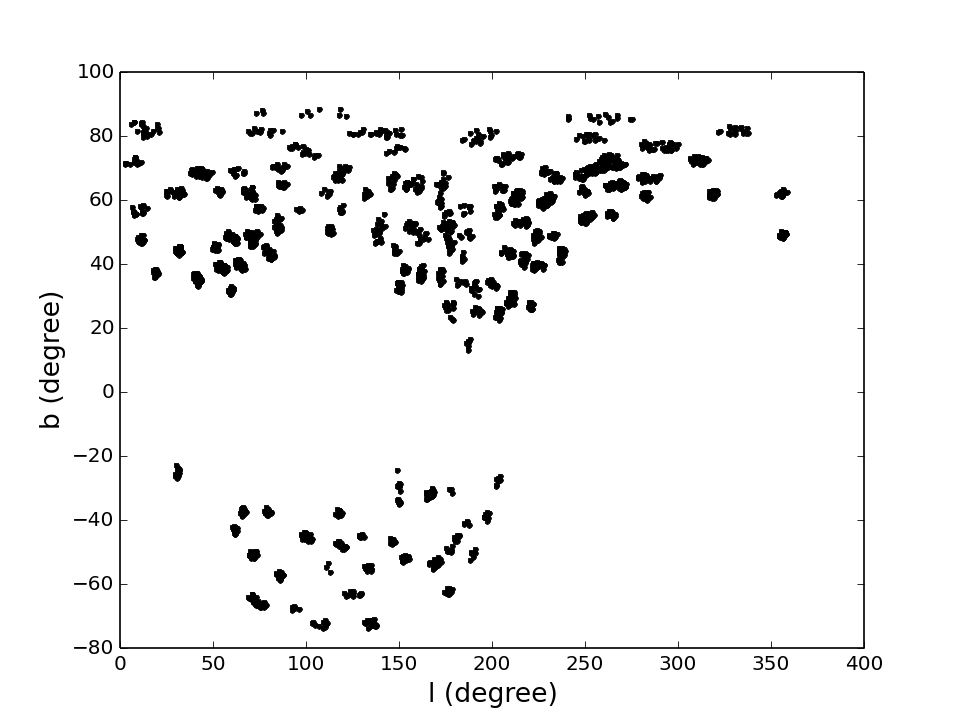
\includegraphics[width=0.5\textwidth,height=0.3\textheight]{skymap_lkg}
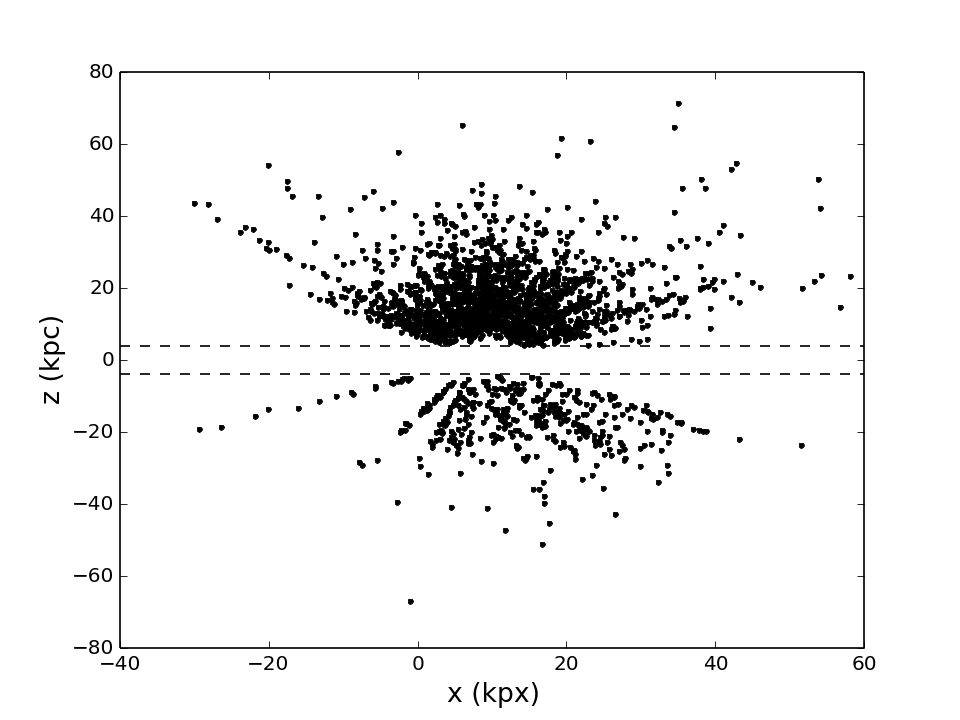
\includegraphics[width=0.5\textwidth,height=0.3\textheight]{xz_lkg}
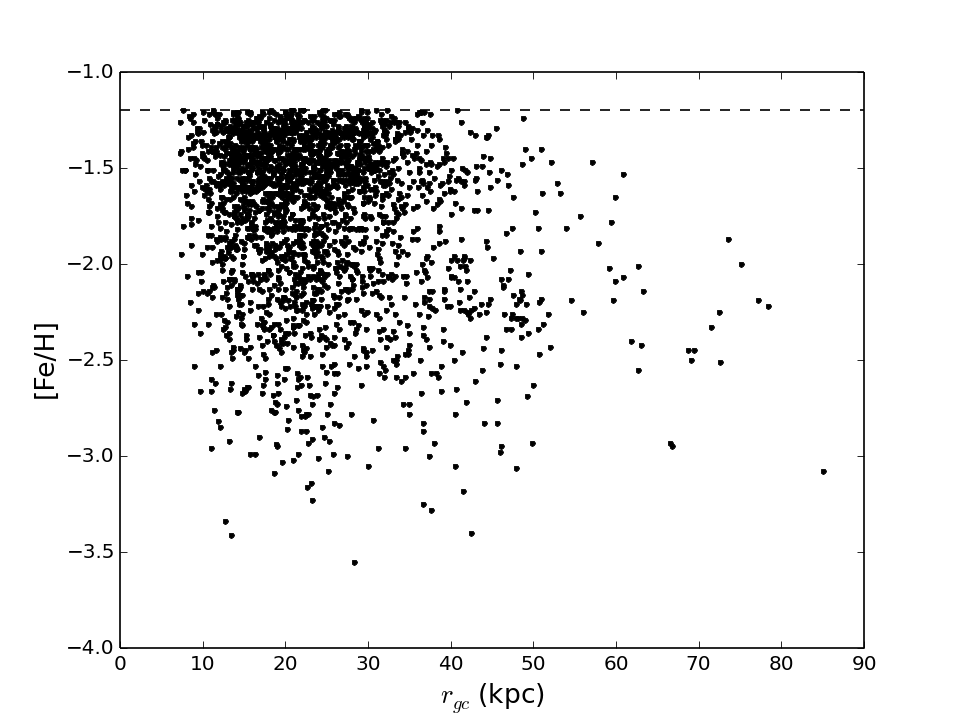
\includegraphics[width=0.5\textwidth,height=0.3\textheight]{rgcfeh_lkg}
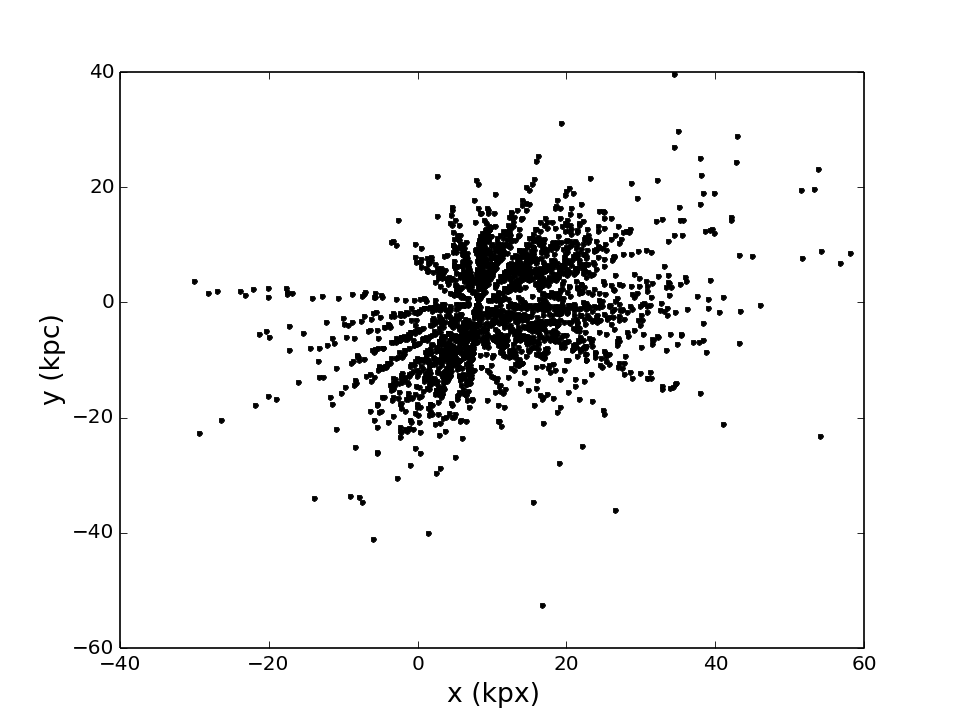
\includegraphics[width=0.5\textwidth,height=0.3\textheight]{xy_lkg}
\caption{(Upper left) The sky coverage and the spatial distributions (right panel) of SEGUE-2 l-color K giants appear to be pencil-beam due to the nature of SEGUE survey. (Lower left) The distribution of metallicities along with the Galactocentric radii shows the mean metallicity is about $\rm -1.75~$dex, and some K giants have metallicities of $\rm \sim -3.5$. The stars with $\rm \feh>-1.2$ and $\rm |z|<4~$kpc are culled because they could belong to the disk.}
\label{f:fkgdistribution}
\end{figure}
\begin{figure}[htbp]
\centering
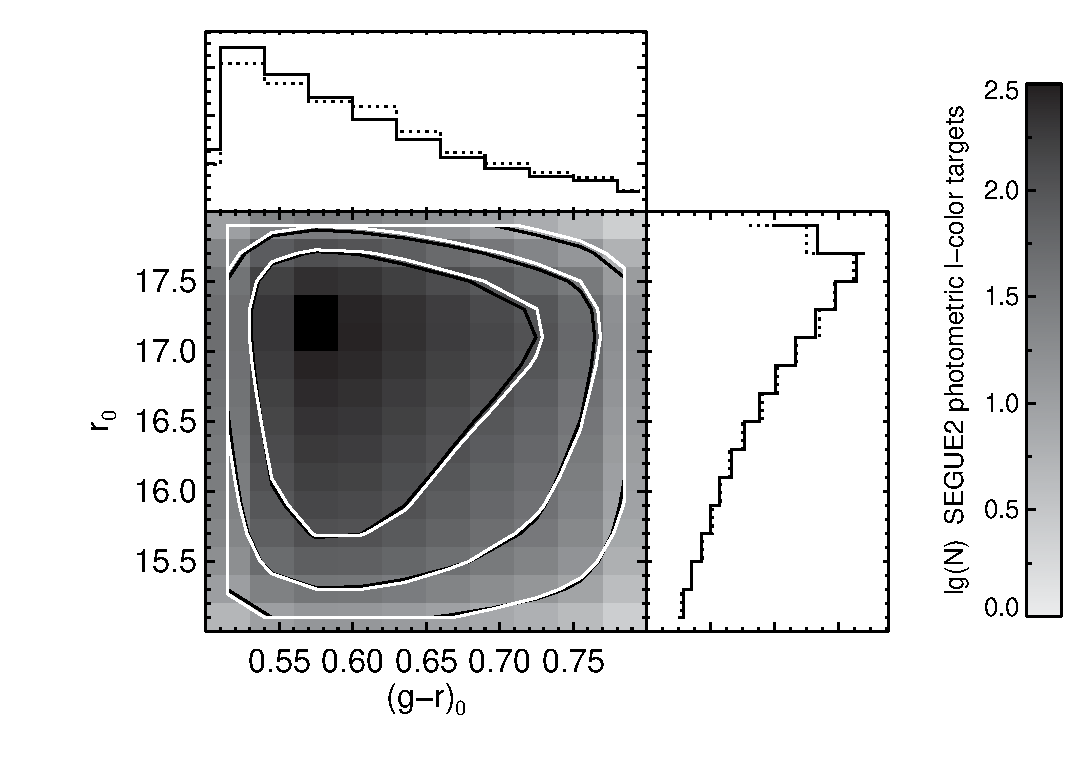
\includegraphics[width=0.48\textwidth,height=0.3\textheight]{gmrvsr0_lctarget}
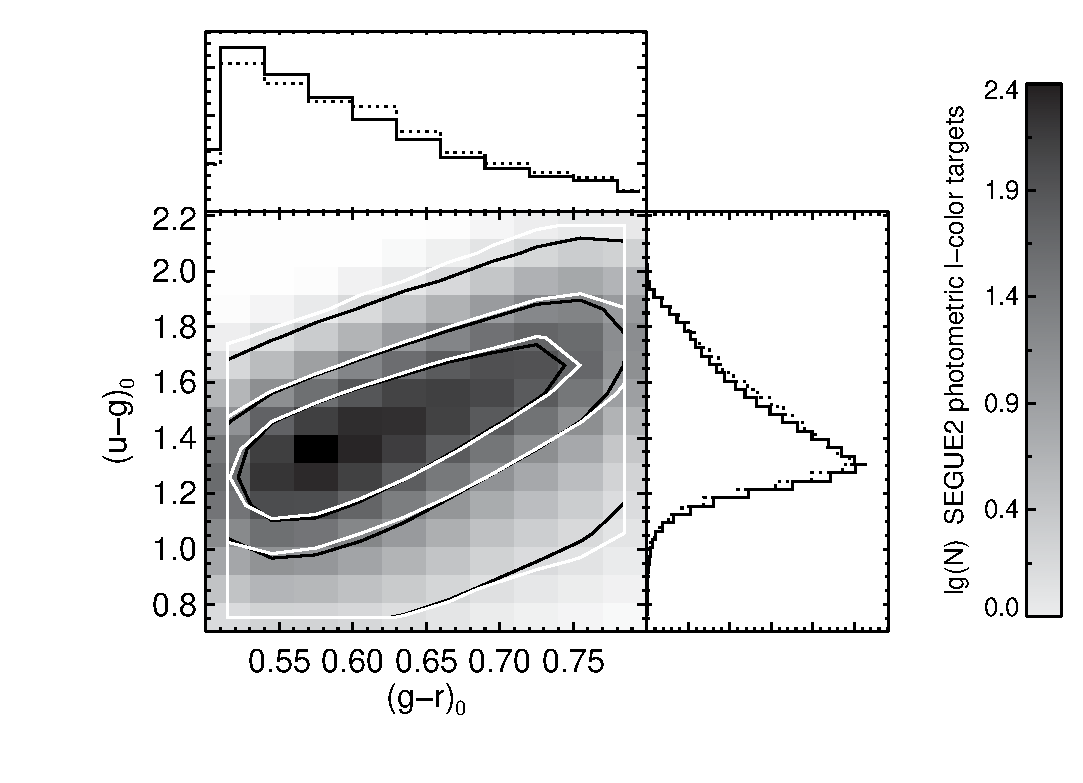
\includegraphics[width=0.48\textwidth,height=0.3\textheight]{gmrvsumg_lctarget}
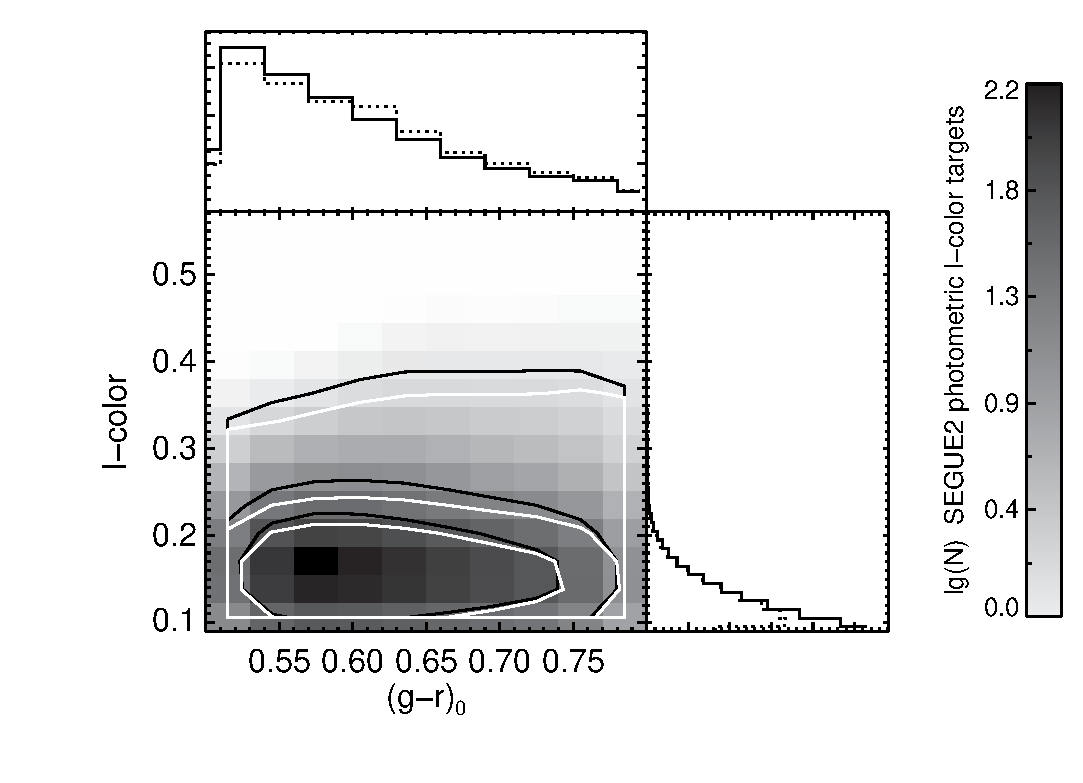
\includegraphics[width=0.48\textwidth,height=0.3\textheight]{gmrvslcolor_lctarget}
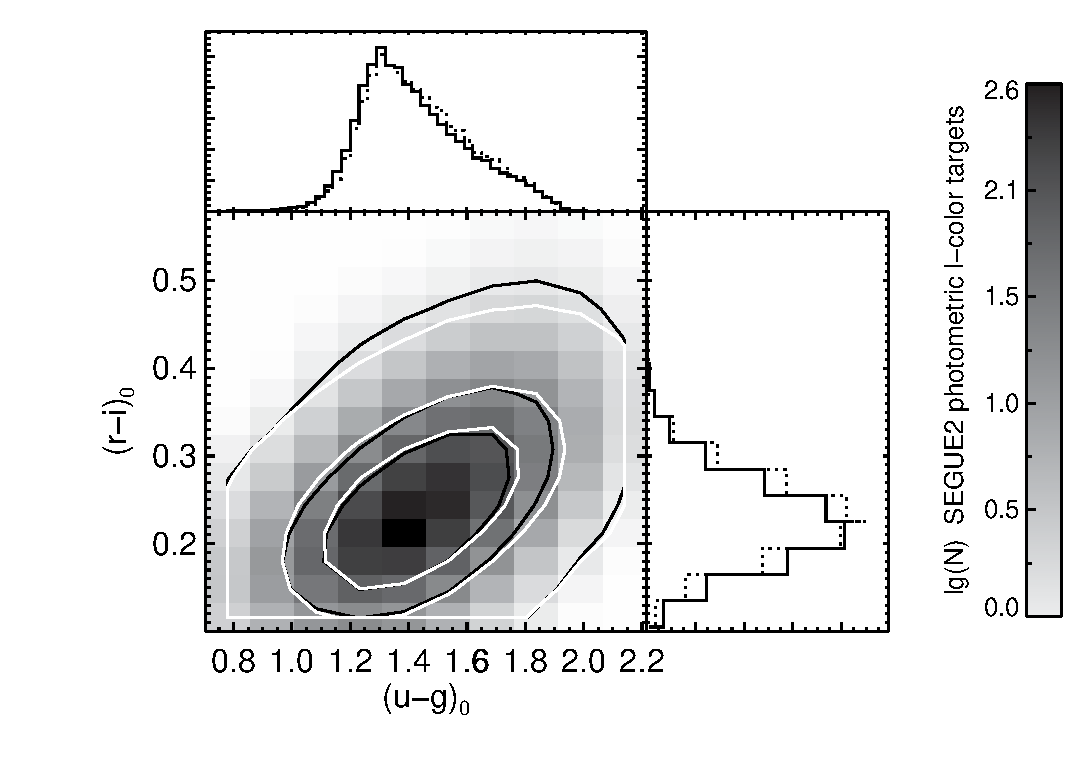
\includegraphics[width=0.48\textwidth,height=0.3\textheight]{umgvsrmi_lctarget}
\caption{Distribution of SEGUE-2 photometric l-color K-giant candidates (gray map, black contours, solid histogram) and the successfully spectroscopic sample (white contours, dotted histogram). The contours contain 68\%, 95\% and 99\% of the distribution. The spectroscopic sampling is relatively fair in colors and magnitudes.}
\label{f:flkgbias}
\end{figure}
\begin{figure}[htbp]
\centering
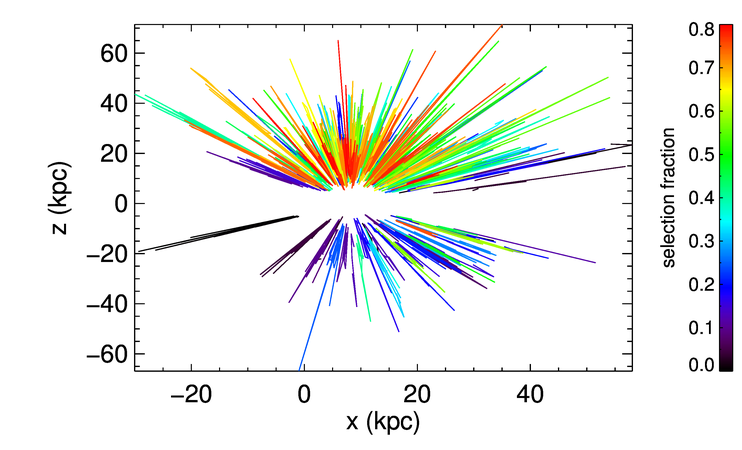
\includegraphics[width=0.48\textwidth,height=0.3\textheight]{sfxzlkg}
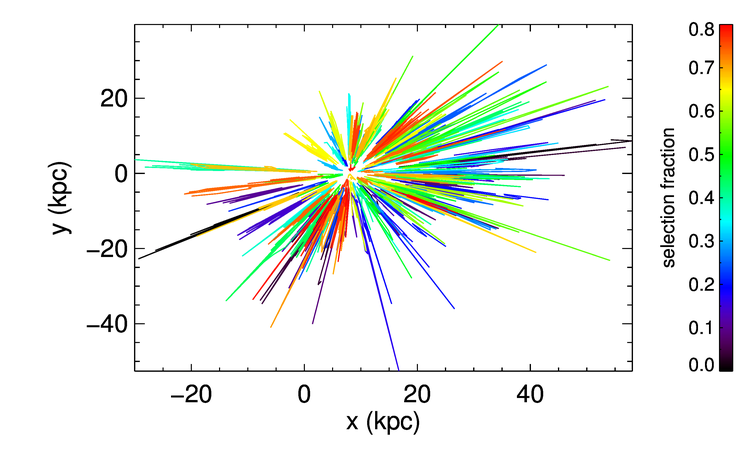
\includegraphics[width=0.48\textwidth,height=0.3\textheight]{sfxylkg}
\caption{The SEGUE-2 selection function of l-color K giants, as a function of Galactic coordinates X and Y (left panel), and of Galactocentric coordinates X and vertical height Z (right panel).}
\label{f:flkgsf}
\end{figure}
\begin{figure}[htbp]
\centering
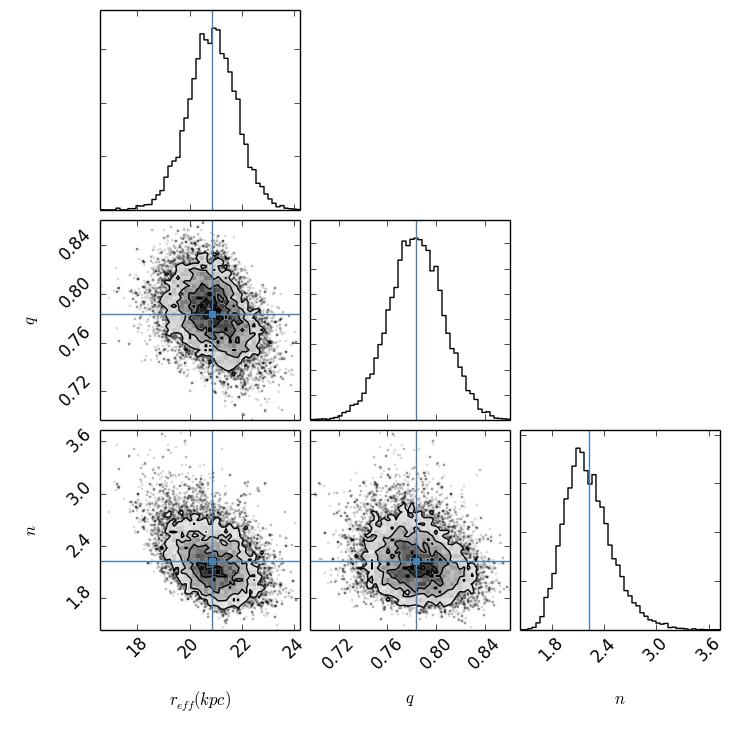
\includegraphics[width=\textwidth]{triangleeinasto}
\caption{The triangle plot shows all the one and two dimensional projections of the posterior probability distributions of parameters $\rm (q,n,r_{eff})$ of Einasto profile. The blue lines and squares mark the best value of each parameter.}
\label{f:feinasto}
\end{figure}
\begin{figure}[htbp]
\centering
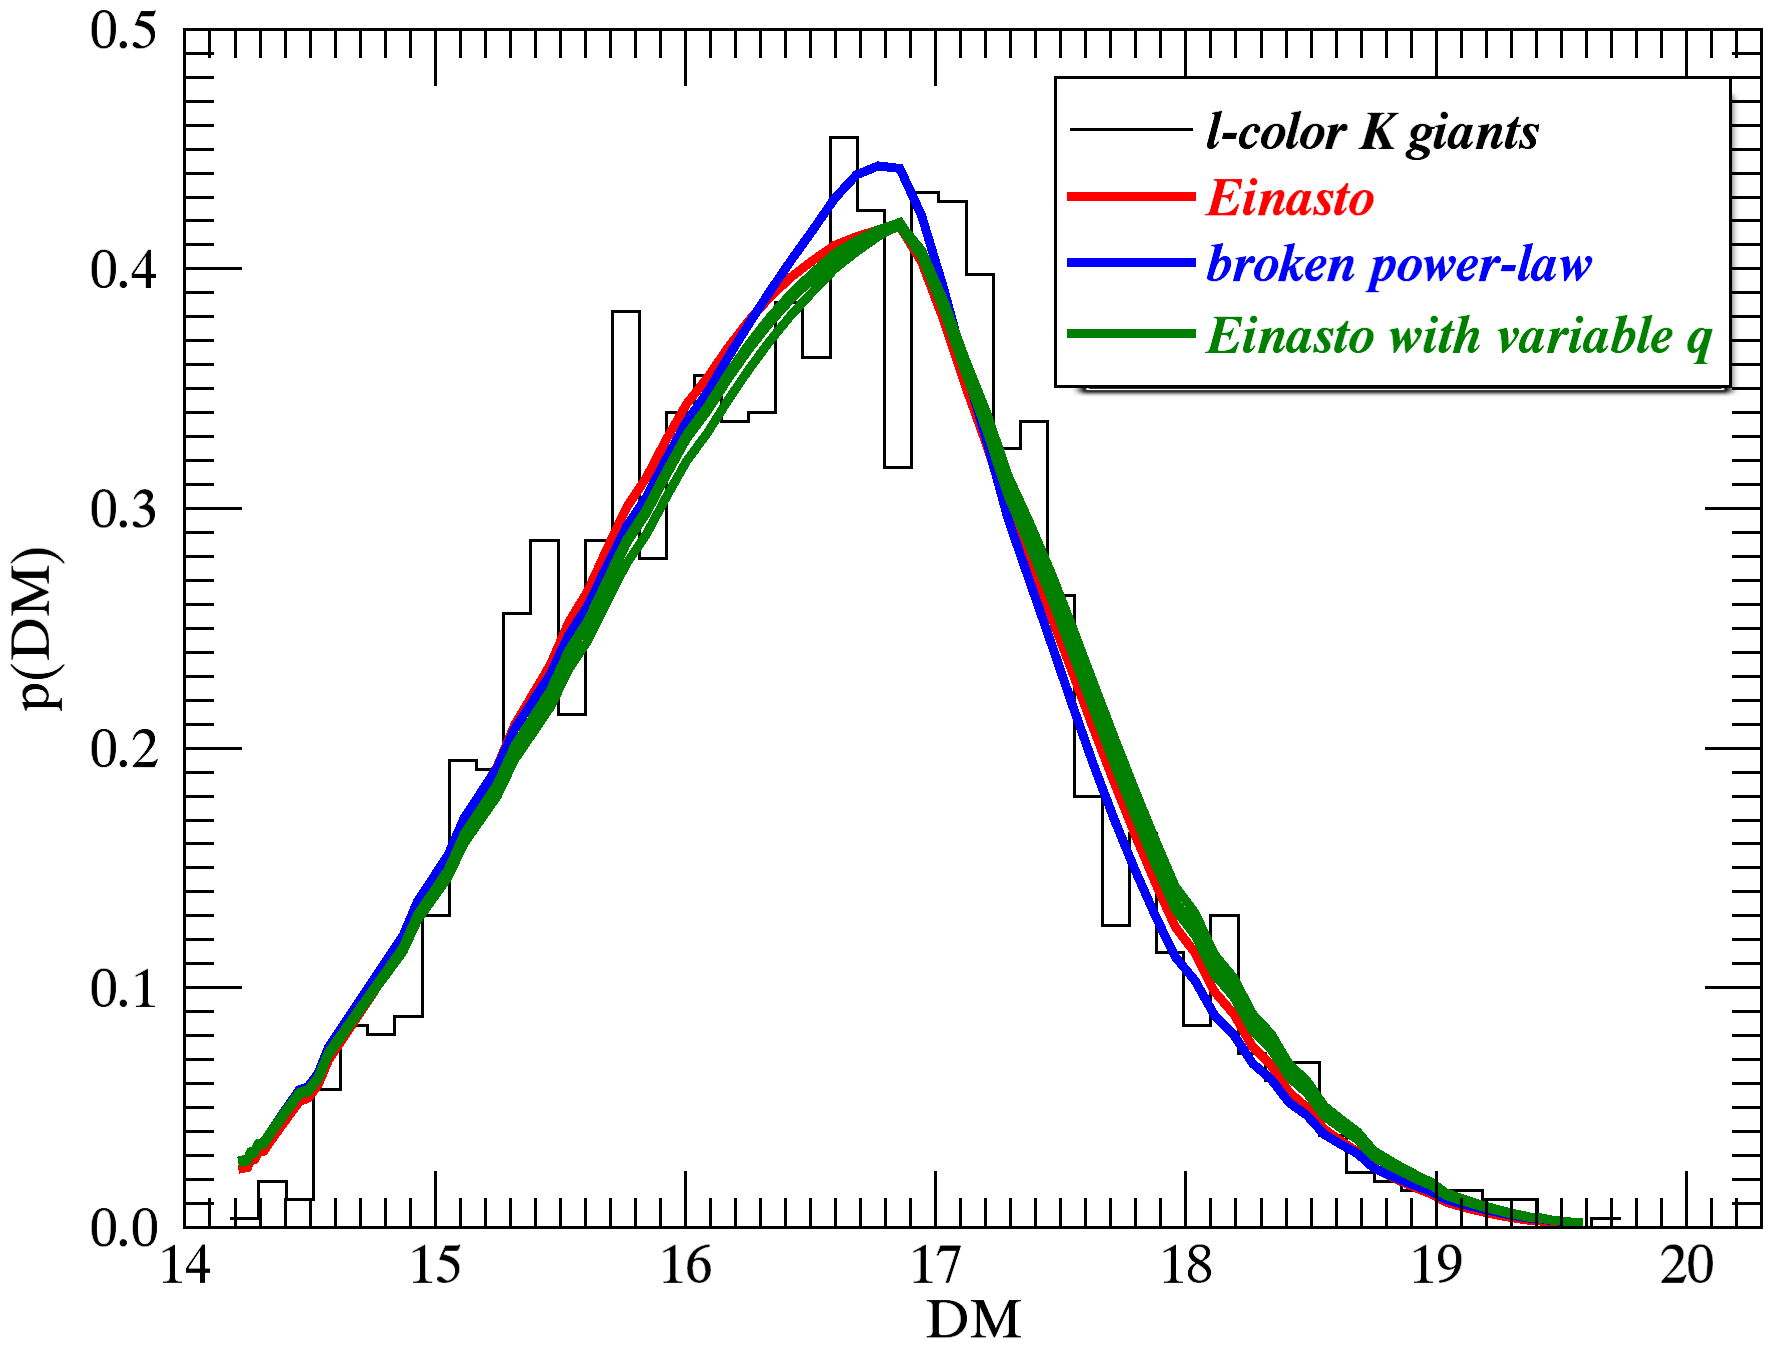
\includegraphics[width=\textwidth]{pdm_hptest_allmodels}
\caption{The comparison between the observed distance-modulus distribution and the predicted distributions by the best-fitting models. All of the best-fitting models fit well.}
\label{f:fpdm}
\end{figure}
\begin{figure}[htbp]
\centering
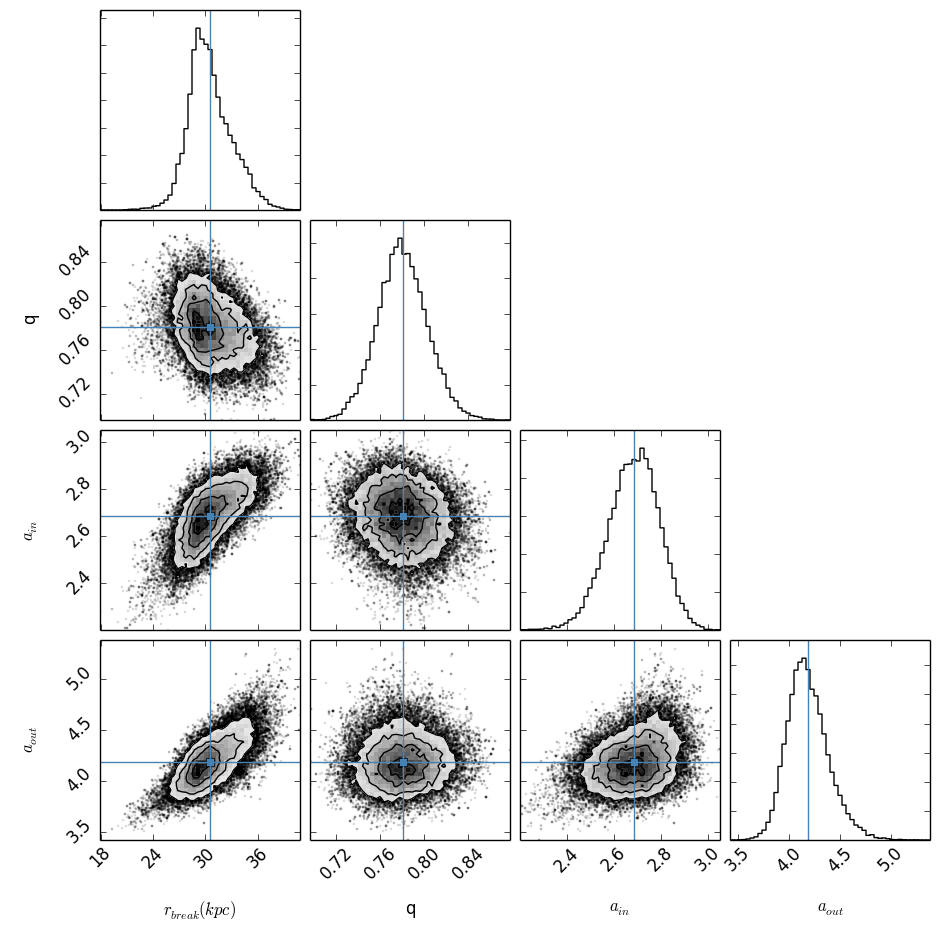
\includegraphics[width=\textwidth]{trianglebpl}
\caption{The triangle plot shows all the one and two dimensional projections of the posterior probability distributions of parameters $\rm (q,\alpha_{in},\alpha_{out},r_{break})$ of the broken power-law profile. The blue lines and squares mark the best value of each parameter.}
\label{f:fbpl}
\end{figure}
\begin{figure}[htbp]
\centering
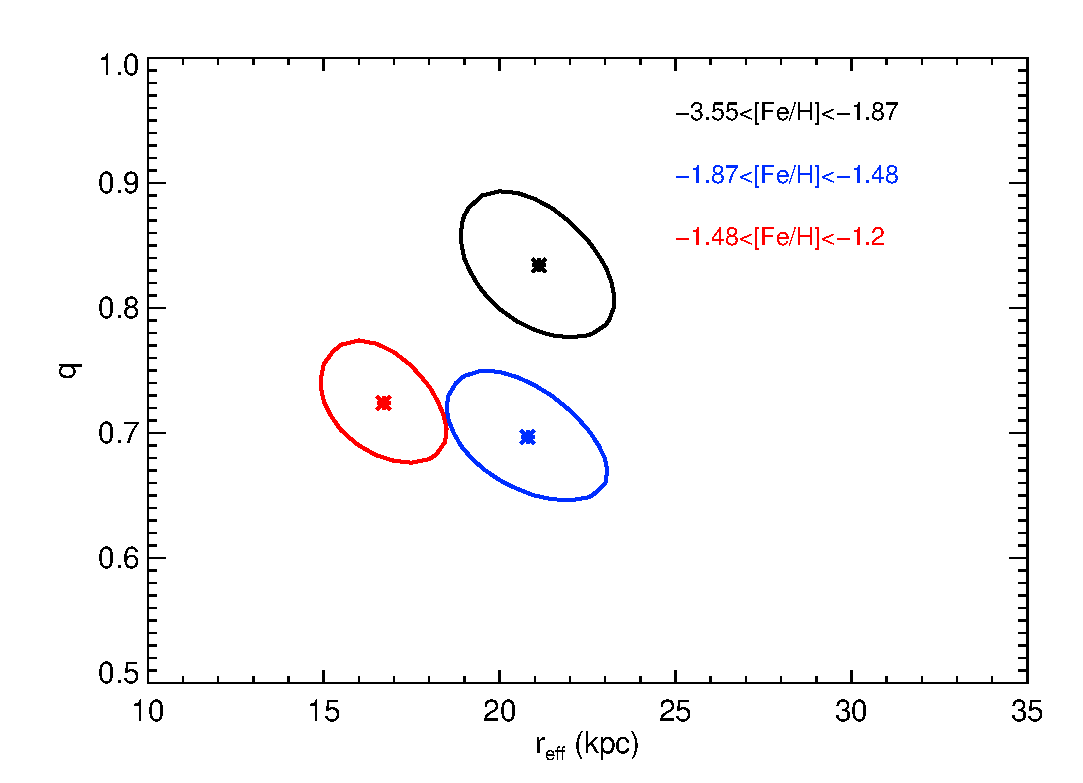
\includegraphics[width=\textwidth]{doublehp_reffqfehbin_Nov12014_einasto_pts96_fixn_contour}
\caption{The best-fit values of flattening and effective radii and their 68\% confidence levels for three sub-samples in different metallicity bins. The shape of the stellar halo has strong dependence on the metallicity, while the radial profile is independent on metallicity.}
\label{f:ffehdependence}
\end{figure}
\begin{figure}[htbp]
\centering
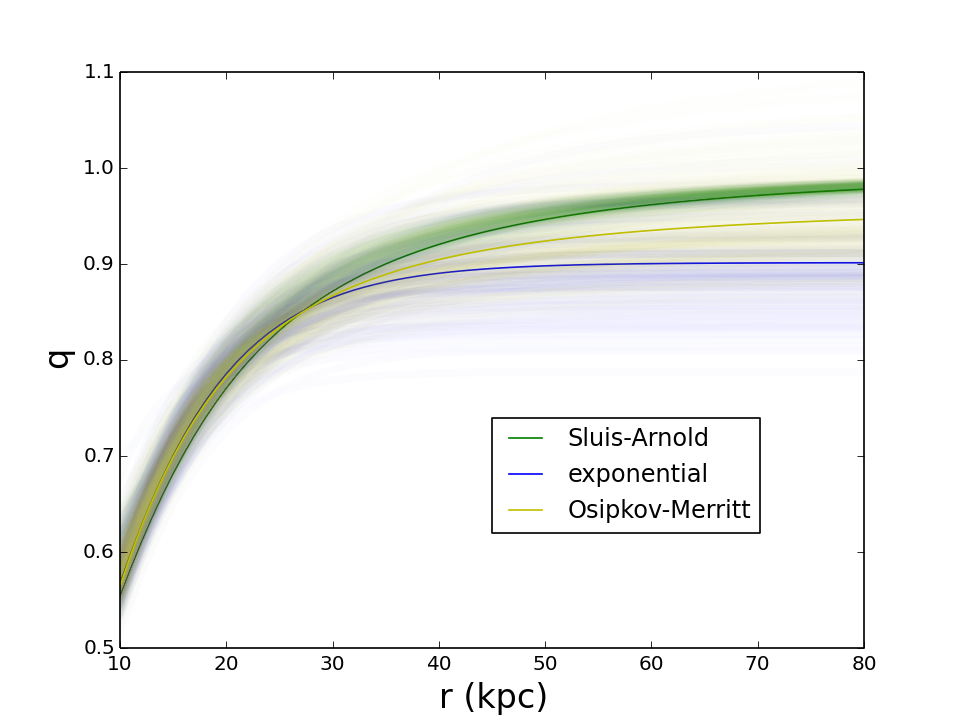
\includegraphics[width=\textwidth]{q_variation}
\caption{The comparison between three models of flattening variation. They are consistent with each other.}
\label{f:fqv}
\end{figure}
\begin{figure}[htbp]
\centering
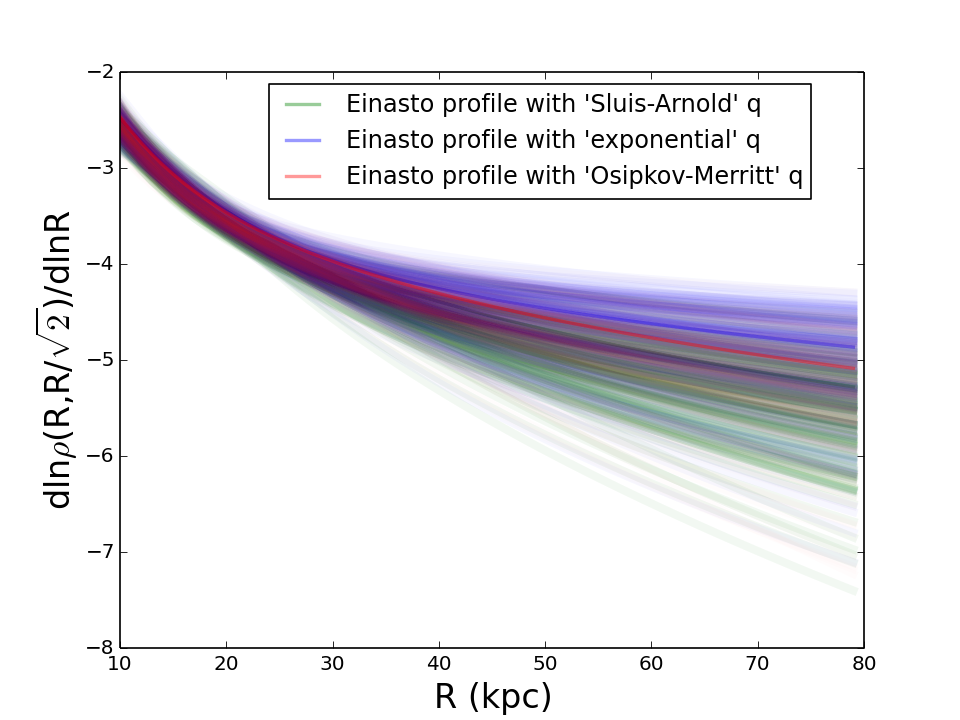
\includegraphics[width=0.9\textwidth,height=0.45\textheight]{density_45d_compareqv}
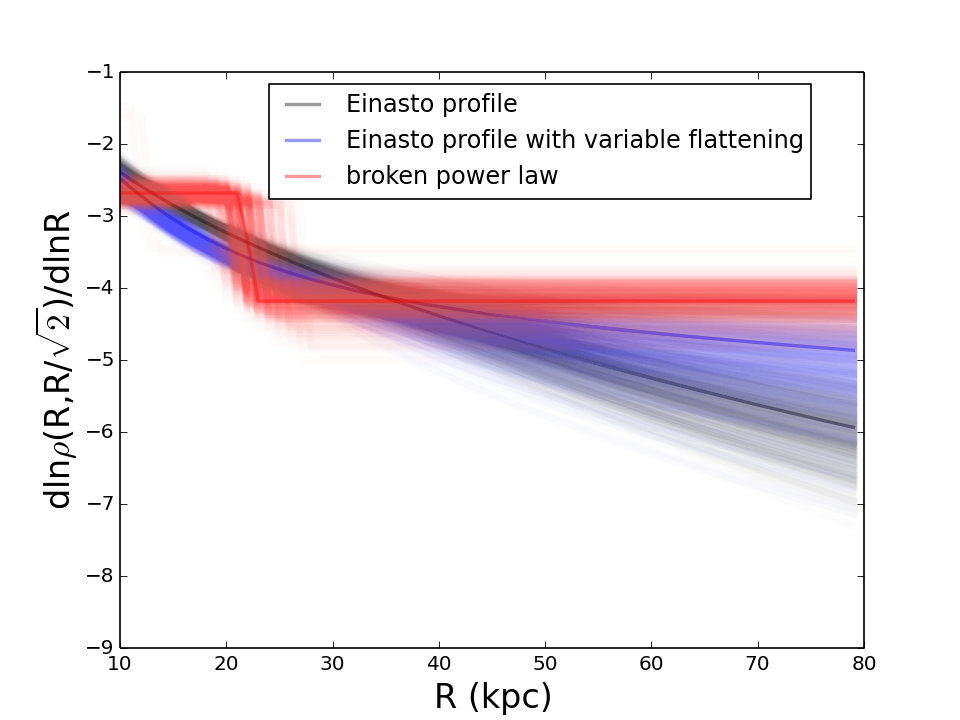
\includegraphics[width=0.9\textwidth,height=0.45\textheight]{density_45d_mcmc}
\caption{(Upper panel) Comparison of the local power-law slope $\rm \frac{dln\nu(R,R/\sqrt{2})}{dlnR}$ for the best-fit Einasto profiles with different functional forms of the flattening variation (Section  \ref{sec:Results_FlatteningVariations}); the lines correspond to radial profiles created from $\rm 200$ samples of the parameter's PDF. (Lower panel) Comparison between the radial profile $\rm \frac{dln\nu(R,R/\sqrt{2})}{dlnR}$ for the best-fit broken power-law with constant flattening (green) and the best-fit triple power-laws with constant flattening (red) and the best-fit Einasto profiles with constant (black) or variable (blue) flattening. Despite the fact that the Einasto profiles in the two cases (black and blue) have effective radii that differ by a factor of two, their radial profiles are very similar within the range constrained by the data. The two dashed lines are the two break radii for triple power-laws. There is no stronger drop beyond 50 kpc. Note that the break radii of double and triple power-laws are in $r_q=(R^2+z^2/q^2)^{0.5}$, but here the x-axis is in $\rm R$.}
\label{f:fdensity}
\end{figure}
\begin{figure}[htbp]
\centering
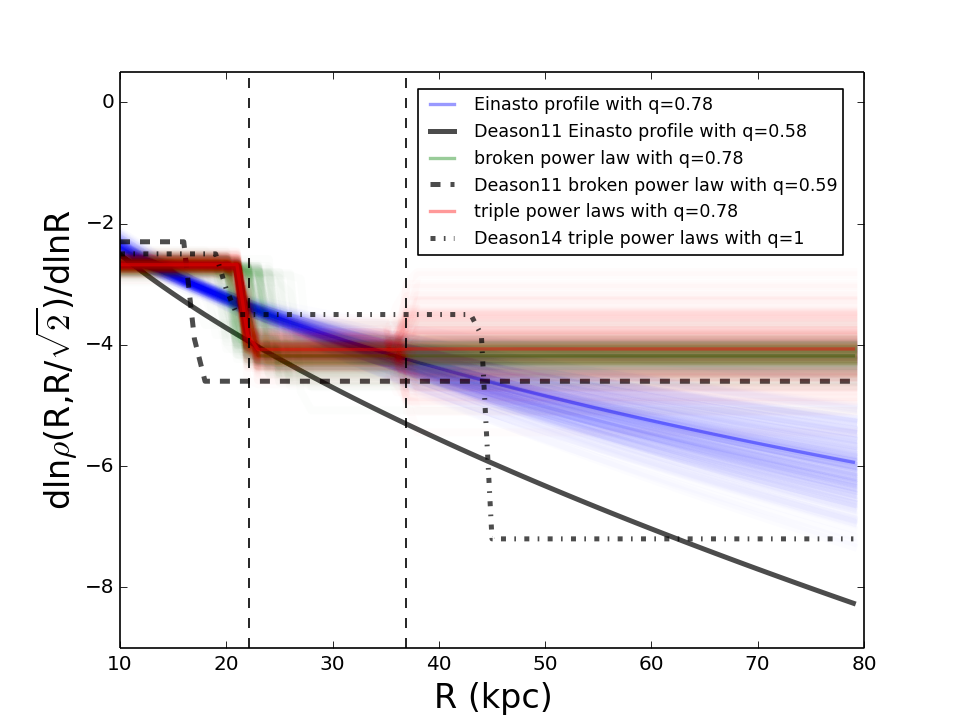
\includegraphics[width=\textwidth]{combinexueanddeason}
\caption{$\rm \frac{dln\nu(R,R/\sqrt{2})}{dlnR}$ for our best-fit broken power-law with constant flattening (green) and best-fit triple power-laws with constant flattening (red) and best-fit Einasto profiles with constant flattening (black) or variable flattening (blue) and the best-fit models of \citet[black]{Deason2011,Deason2014}. The two vertical dashed lines indicate the two break radii of triple power-laws.}
\label{f:fdensitycompare}
\end{figure}

\begin{table}
\tiny
\begin{threeparttable}
\caption{A summary of our best-fitting models}
\begin{tabularx}{1.1\textwidth}{llll}
\hline\hline \\
Model & Parameters & $\rm N_p$ & $ln(\mathscr{L})$ \\
\hline \\
Einasto & $\rm n=2.2\pm0.3$, $\rm r_{eff}=21\pm1~kpc$, $\rm q=0.78\pm0.02$ & 3 & --18093\\ 
Broken power-law & $\rm \alpha_{in}=2.7\pm0.1$, $\rm \alpha_{out}=4.2\pm0.2$, $\rm r_{break}=30\pm3kpc$,$q=0.78\pm0.02$ & 4 & --18090 \\ 
Triple power-laws & $\rm \alpha_{1}=2.7\pm0.1$, $\rm \alpha_{2}=4.1\pm0.2$, $\rm \alpha_{3}=4.1\pm0.5$, $q=0.78\pm0.02$, $\bm{r_{break1}=30kpc}$, $\bm{r_{break2}=50kpc}$ & 3 & --18065\\  
Einasto-exponential q(r) & $\rm n=5.4\pm1.8$, $\rm r_{eff}=7\pm3~kpc$, $\rm q_0=0.3\pm0.1$, $\rm q_{inf}=0.9\pm0.04$, $\rm r_{0}=8\pm2~kpc$ & 5 & --18077 \\ 
Einasto-Osipkov-Merritt q(r) & $\rm n=4.6\pm1.5$, $\rm r_{eff}=8\pm3~kpc$, $\rm q_0=0.2\pm0.1$, $\rm q_{inf}=0.96\pm0.05$, $\rm r_{0}=15\pm3~kpc$ & 5 & --18077 \\ 
Einasto-Sluis-Arnold q(r) & $\rm n=4.2\pm1.5$, $\rm r_{eff}=8\pm3~kpc$, $\rm q_0=0.3\pm0.1$, $\rm r_{0}=6\pm3~kpc$ & 4 & --18077 \\ 
\hline
\end{tabularx}
\begin{tablenotes}
\item  We give the type of model, the best-fitting parameters of the model, the number of free parameters, the log-likelihood for the best-fitting model. Parameters which are kept fixed are highlighted in bold.
\end{tablenotes}
\end{threeparttable}
\end{table}

\end{document}
